\documentclass{beamer}

\mode<presentation> {
\usetheme{Madrid}
}

\usepackage{graphicx} % Allows including images
\usepackage{booktabs} % Allows the use of \toprule, \midrule and \bottomrule in tables
\usepackage{listings}
\usepackage{multicol}

\title[HawkTracer profiler]{HawkTracer profiler}

\author{Marcin Kolny} % Your name
\institute[Amazon Prime Video]
{
  Amazon Prime Video \\
  \textit{marcin.kolny@gmail.com}
}
\date{February 2, 2020}
\definecolor{darkgreen}{rgb}{0,0.6,0}
\lstset{language=C++,
                basicstyle=\ttfamily,
                keywordstyle=\color{blue}\ttfamily,
                stringstyle=\color{red}\ttfamily,
                commentstyle=\color{darkgreen}\ttfamily,
                morecomment=[l][\color{magenta}]{\#}
}
\begin{document}

\begin{frame}
  \titlepage
\end{frame}

% \begin{frame}[fragile]
%   \frametitle{What is profiler?}
%   \textbf{Performance profiling} - analyzing performance of the application
%   \vspace{1em}
%   \begin{itemize}
%     \item sampling(statistical) profiler - periodically polls the application to get data(e.g. callstacks, CPU usage)
%     \begin{itemize}
%       \item insignificant overhead
%       \item example: perf
%     \end{itemize}
%     \vspace{1em}
%   \item instrumentation profiler - requires from developer to place instructions in the code to collect required data
%     \begin{itemize}
%       \item more accurate data
%       \item example: LTTng, HawkTracer
%     \end{itemize}
%   \end{itemize}
% \end{frame}

\begin{frame}[fragile]
  \frametitle{Why do we need another profiler?}
  \begin{minipage}[c]{0.65\linewidth}
  \textbf{Environment:}
  \begin{itemize}
    \item Limited access to the device
    \item Lack of development tools
    \item Various low-end platforms
    \item Various languages (C++ for native, Lua and JavaScript for scripted)
  \end{itemize}
  \end{minipage}
  \begin{minipage}[c]{0.3\linewidth}
    
\includegraphics[width=1\textwidth]{img/prime-video.png}
  \end{minipage}
  \pause \\
  \vspace{0.7em}
  \textbf{HawkTracer features:}
  \begin{itemize}
    \item User space \& instrumentation based
    \item Written in C (and C++) but available for other languages
    \item Built-in to executable as a library ("install app" only)
    \item Low cost of porting (to SmartTVs/Consoles/Streaming Sticks/...)
    \item Measure timings as well as arbitrary resource usage
    \item Low overhead (lock-free when possible)
    \item Consistent user experience across all supported platforms
  \end{itemize}
\end{frame}

\begin{frame}[fragile]
  \frametitle{High Level architecture}
  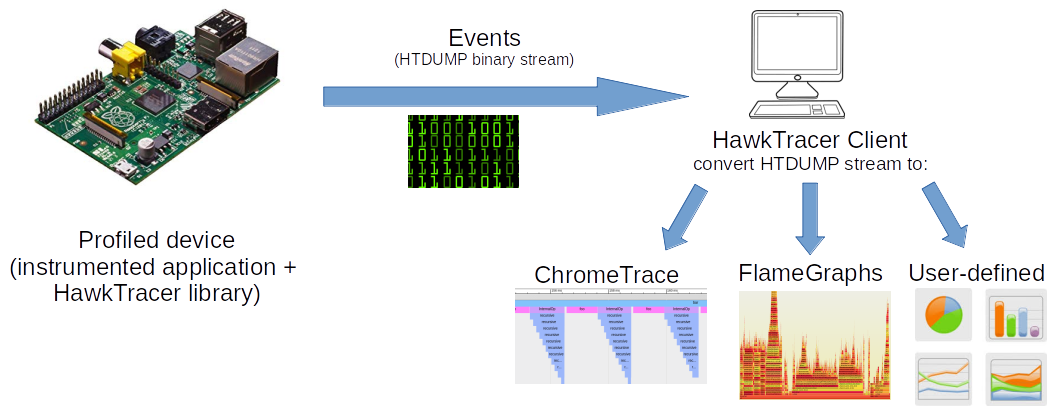
\includegraphics[width=1\textwidth]{img/high-level-architecture.png} \\
  \begin{itemize}
    \item Event - base data unit (predefined or user-defined event types)
    \item HTDUMP stream - binary stream (sent to a client over TCP / File / user-defined protocol)
    \item Client - converts HTDUMP stream to human-readable representation
  \end{itemize}
\end{frame}

\begin{frame}[fragile]
  \frametitle{Data flow / component diagram}
  \begin{center}
    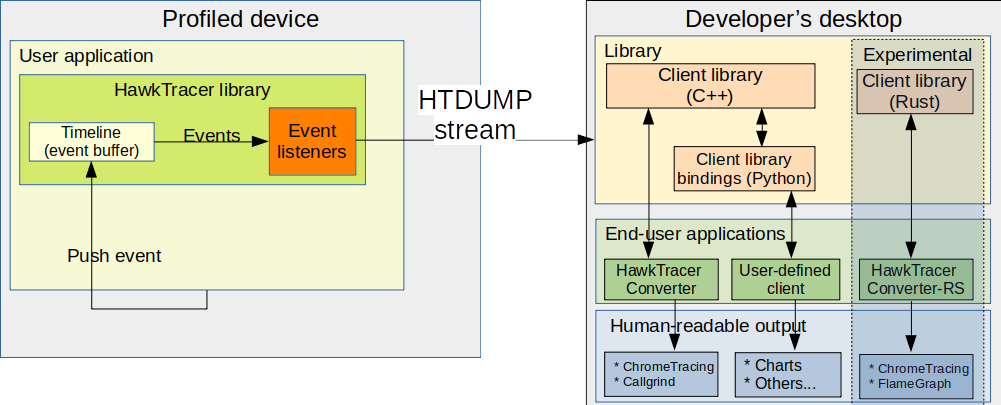
\includegraphics[width=0.9\textwidth]{img/data-flow.png}
    \begin{itemize}
      \item Timeline - event buffer, lock-free or thread-safe (up to the usecase)
      \item Event Listener - processes batch of events (e.g. store to file, send over TCP/IP)
      \item Client library - converts HTDUMP stream to list of Event structures
    \end{itemize}
  \end{center}
\end{frame}

\begin{frame}[fragile]
  \frametitle{Global Timeline}
  \begin{itemize}
    \setlength\itemsep{0.4em}
    \item predefined in the HawkTracer library
    \item recommended for most of the usecases
    \item per-thread instance (no locks required)
    \item \lstinline{ht_global_timeline_get()}
  \end{itemize}

\end{frame}

\begin{frame}[fragile]
  \frametitle{Defining event types}
  \fontsize{9pt}{1}\selectfont
  \begin{itemize}
    \item C structure with arbitrary fields
    \item support for inheritance
    \item runtime structure introspection (using MKCREFLECT library)
  \end{itemize}
  \begin{lstlisting}[language=C++,basicstyle=\tiny]
HT_DECLARE_EVENT_KLASS(
  MyEvent, // Event class name
  HT_Event, // Base event
  (INTEGER, uint8_t, field_1), // field definition (type, C type, field name)
  (STRING, char*, field_2)     // field definition (type, C type, field name)
  // Other fields...
)
  \end{lstlisting}

  Converts to C structure and a few helper methods:
  \begin{multicols}{2}
    \begin{lstlisting}[language=C++,basicstyle=\tiny]
typedef struct {
  HT_Event base;
  uint8_t field_1;
  char* field_2;
} MyEvent;

// Serializes event to HTDUMP format
size_t ht_MyEvent_fnc_serialize(
  HT_Event* event, HT_Byte* buffer);
    \end{lstlisting}
    \columnbreak
    \begin{lstlisting}[language=C++,basicstyle=\tiny]
typedef struct {
  HT_EventKlass* klass;
  uint64_t timestamp_ns;
  uint64_t event_id;
} HT_Event;

// Information about the class structure
MKCREFLECT_TypeInfo*
  mkcreflect_get_MyEvent_type_info(void);
    \end{lstlisting}
  \end{multicols}
  \vspace{-0.7em}
  Pushing event to a timeline:
  \begin{lstlisting}[language=C++,basicstyle=\tiny]
  HT_TIMELINE_PUSH_EVENT(timeline, MyEvent, 28, "Hello World!");
  \end{lstlisting}

\end{frame}

\begin{frame}[fragile]
  \frametitle{HTDUMP Event stream}
  \fontsize{10pt}{7.2}\selectfont
  \begin{itemize}
    \item \textbf{Metadata stream} - information about event types \\
      {\tiny (transferred as \lstinline{HT_EventKlassInfoEvent} and \lstinline{HT_EventKlassFieldInfoEvent} events)}
      \begin{lstlisting}[language=C++,basicstyle=\tiny]
HT_EventKlassInfoEvent {               //     33 bytes
    "type": U32(2)                     // 02 00 00 00
    "timestamp": U64(394021837478301)  // 9D 19 A8 5B 5C 66 01 00
    "id": U64(38)                      // 26 00 00 00 00 00 00 00
    "info_klass_id": U32(9)            // 09 00 00 00
    "event_klass_name": Str("MyEvent") // 4D 79 45 76 65 6E 74 00
    "field_count": U8(3)               // 03
}
HT_EventKlassFieldInfoEvent {          //     49 bytes
    "type": U32(3)                     // 03 00 00 00
    "timestamp": U64(394021837479489)  // 41 1E A8 5B 5C 66 01 00
    "id": U64(40)                      // 28 00 00 00 00 00 00 00
    "info_klass_id": U32(9)            // 09 00 00 00
    "field_type": Str("uint8_t")       // 75 69 6E 74 38 5F 74 00
    "field_name": Str("field_1")       // 66 69 65 6C 64 5F 31 00
    "size": U64(1)                     // 01 00 00 00 00 00 00 00
    "data_type": U8(99)                // 63
}
// ...
      \end{lstlisting}

  \item Events stream
    \begin{lstlisting}[language=C++,basicstyle=\tiny]
MyEvent {                              //     34 bytes
  "type": U32(9)                       // 09 00 00 00
  "timestamp": U64(394021837504177)    // B1 7E A8 5B 5C 66 01 00
  "id": U64(42)                        // 2A 00 00 00 00 00 00 00
  "field_1": U8(28)                    // 1C
  "field_2": Str("Hello World!")       // 48 65 6C 6C 6F 20 57 6F 72 6C 64 21 00
}
    \end{lstlisting}
  \end{itemize}
\end{frame}

% \begin{frame}
%   \frametitle{Demo 1 - Hello World!}
%   \begin{center}
%     \Huge Demo 1 - Hello World!
%   \end{center}
% \end{frame}

\begin{frame}[fragile]
  \frametitle{Measuring time - predefined events}
  \begin{itemize}
    \item C / C++
      \begin{lstlisting}[language=C++,basicstyle=\tiny]
  void foo()
  {
    HT_TRACE_FUNCTION(timeline);
    // HT_G_TRACE_FUNCTION() for Global Timeline
    // ...
    { // new scope
      HT_TRACE(timeline, "custom label");
      // HT_G_TRACE("custom label") for Global Timeline
      // use HT_TRACE_OPT_* for better performance
    }
  }
    \end{lstlisting}
  \item Python
    \begin{lstlisting}[language=Python,basicstyle=\tiny]
  from hawktracer.core import trace

  @trace  # uses Global Timeline
  def foo():
    pass
    \end{lstlisting}
  \item Rust
    \begin{lstlisting}[language=C,basicstyle=\tiny]
  #[hawktracer(trace_this)] // uses Global Timeline
  fn method_to_trace() {
    // ...
    { // new scope
      scoped_tracepoint!(_custom_label);
      // ...
    }
  }
    \end{lstlisting}
  \end{itemize}
\end{frame}

% \begin{frame}
%   \frametitle{Demo - Time measurements}
%   \begin{center}
%     \Huge Demo - Time measurements
%   \end{center}
% \end{frame}

\begin{frame}
  \frametitle{Demo - Real-time data stream}
  \begin{center}
    \Huge Demo - Real-time data stream \\
    \LARGE Writing custom client
    \vspace{1em} \\
    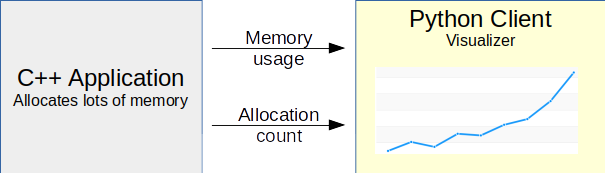
\includegraphics[width=0.8\textwidth]{img/resource-usage.png} \\
  \end{center}
\end{frame}

\begin{frame}
  \frametitle{Demo - Cross-language project}
  \begin{center}
    \Huge Demo - Cross-language project
    \vspace{0.2em} \\
    \large Rust \& Python \& C
    \vspace{1em} \\
    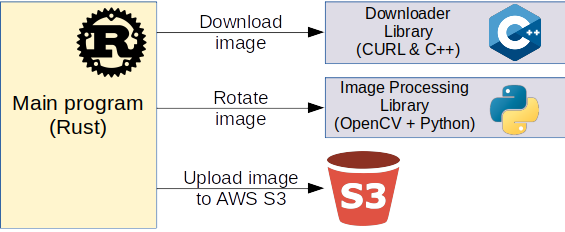
\includegraphics[width=0.8\textwidth]{img/rotate-diagram.png} \\
  \end{center}
\end{frame}

\begin{frame}
  \frametitle{Future improvements}
  \begin{itemize}
    \item Generic data viewer
    \item CTF support
    \item Bindings for more languages (JavaScript)
    \item Allow custom event type definitions from bindings
    \item ...
  \end{itemize}
\end{frame}


\begin{frame}

  \frametitle{Thank you!}
  \fontsize{10pt}{1}\selectfont
  \begin{minipage}[c]{0.7\linewidth}
    \begin{itemize}
      \setlength\itemsep{0.8em}
      \item marcin.kolny@gmail.com
      \item HawkTracer website: \\
        {\scriptsize (entry point, community, how to get involved)}
        \href{https://www.hawktracer.org}{www.hawktracer.org} \\
      \item Documentation: \\
        {\scriptsize (reference, tutorials, design concepts, integration)}
        \href{https://www.hawktracer.org/doc}{www.hawktracer.org/doc}
      \item Code repository: \\
      \begin{itemize}
        \setlength\itemsep{0.8em}
        \item HawkTracer Core:\\
          \href{https://github.com/amzn/hawktracer}{github.com/amzn/hawktracer}
        \item HawkTracer Converter (Rust): \\
          \href{https://github.com/loganek/hawktracer-converter}{github.com/loganek/hawktracer-converter}
        \item HawkTracer Rust bindings: \\
        \href{https://github.com/AlexEne/rust\_hawktracer}{github.com/AlexEne/rust\_hawktracer}
      \end{itemize}
    \end{itemize}
  \end{minipage}
  \begin{minipage}[c]{0.25\linewidth}
    \begin{center}
      \vspace{1em}
      
\includegraphics[width=4em]{img/documentation.png} \\
      \vspace{1.5em}
      
\includegraphics[width=5em]{img/github.png} \\
      \vspace{1.5em}
      
\includegraphics[width=5em]{img/rust.png}
    \end{center}
  \end{minipage}
\end{frame}

\end{document}
